\chapter{सांख्यिकीय ऊष्मागतिकी के अनुप्रयोग}\label{ch:b3:statistical-thermo-applied}

सबसे अच्छी तरह ऊष्मारोधित टंकी में रखा द्रव हाइड्रोजन भी उबलकर उड़ता रहता है, और
द्रवण के बाद के पहले दिनों में वह दीवारों से रिसती ऊष्मा की व्याख्या से कहीं
तेज़ी से उड़ता है। ऊष्मा द्रव के भीतर से आती है। हाइड्रोजन
अणु दो रूपों में होते हैं, जो केवल अपने दोनों प्रोटॉनों के चक्रणों के आपेक्षिक
अभिविन्यास में भिन्न होते हैं और जो एक-दूसरे में केवल बहुत
धीरे बदलते हैं; \qty{20}{K} पर एक रूप का दूसरे में रूपांतरण द्रव को वाष्पित करने के लिए
आवश्यक ऊष्मा से अधिक ऊष्मा मुक्त करता है। यह अध्याय
\cref{ch:b3:partition-functions} के विभाजन फलनों को ऊष्मा धारिताओं पर,
इन नाभिकीय-चक्रण समावयवियों पर और उस एन्ट्रॉपी पर लागू करता है जो कुछ क्रिस्टल 0 K पर बनाए रखते हैं,
फिर केवल स्पेक्ट्रमी आँकड़ों से साम्य स्थिरांक और समस्थानिक प्रभाव
परिकलित करता है।

\begin{recall}
\Cref{ch:b3:partition-functions} ने \omterm{def:b3:partition-functions:partition-function}{आण्विक विभाजन फलन} और उसके
चार गुणक बनाए, और उससे $U$, $S$ और $G$ व्युत्पन्न किए। द्वितीय वर्ष के खंड ने
मानक साम्य स्थिरांक को मानक अभिक्रिया गिब्स ऊर्जा से जोड़ा,
$\Delta_rG^\circ = -RT\ln K^\circ$, और वांट हॉफ़ समीकरण स्थापित किया;
\cref{ch:b3:many-electron-atoms} ने बताया कि दो सर्वसम फ़र्मिऑनों के विनिमय पर
तरंग फलन चिह्न बदलता है; \cref{ch:b3:rovibrational-spectroscopy} ने
\ce{H2}-सदृश अणुओं के घूर्णी रामन स्पेक्ट्रम में रेखा-तीव्रताओं का 3:1 एकांतरण पाया।
विद्यालय के खंड के कक्षा 9 वाले भाग ने समस्थानिक परिभाषित किए।
\end{recall}

\begin{omfigure}
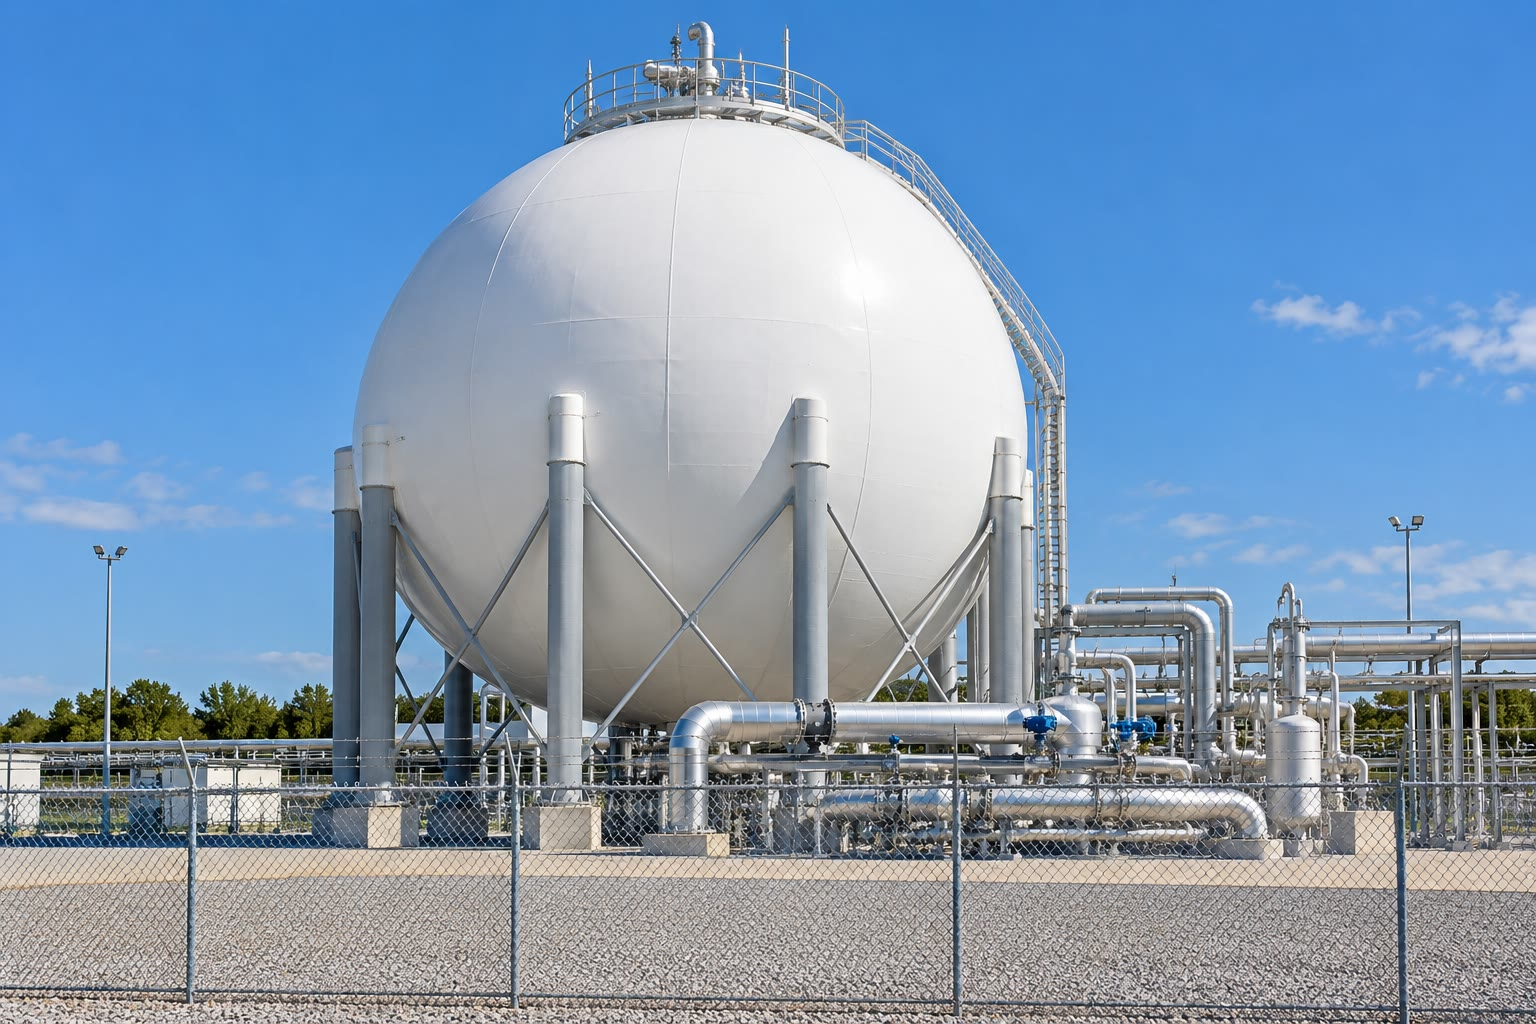
\includegraphics[width=0.6\linewidth]{images/book4/ai/b3-11-lh2-tank.jpg}

{\small द्रव हाइड्रोजन के लिए एक गोलाकार टंकी। \qty{20}{K} पर द्रव के भीतर
हाइड्रोजन के एक नाभिकीय-चक्रण रूप के दूसरे में धीमे रूपांतरण से उत्पन्न ऊष्मा
बाहर से रिसकर आने वाली ऊष्मा से अधिक हो सकती है।}
\end{omfigure}

\section{गैसों की ऊष्मा धारिताएँ}

स्थिर आयतन पर ऊष्मा धारिता $C_V = (\partial U/\partial T)_V$ है, और
\cref{thm:b3:partition-functions:internal-energy} के साथ हर प्रकार की गति
अलग से योगदान देती है। दो सीमाएँ सब कुछ नियंत्रित करती हैं।

\begin{theorem}[समविभाजन प्रमेय]\label{thm:b3:statistical-thermo-applied:equipartition}
जब किसी गति के ऊर्जा स्तर $kT$ की तुलना में पास-पास हों, तो उसकी ऊर्जा का हर
पद जो किसी निर्देशांक या संवेग में द्विघाती है, अणु की माध्य ऊर्जा में
$\frac12kT$ का योगदान देता है, अतः मोलर ऊष्मा
धारिता में $\frac12R$ का। यही कथन \emph{समविभाजन प्रमेय}\index{समविभाजन प्रमेय} है।
\end{theorem}

\begin{proof}[आंशिक उपपत्ति]
चिरसम्मत सीमा में किसी गति की अवस्थाओं पर योग एक
समाकल बन जाता है, और द्विघाती पद $a u^2$ गुणक $\int\eu^{-\beta au^2}\dd u =
\sqrt{\pi/\beta a}$ का योगदान देता है, जो $\beta^{-1/2}$ के समानुपाती है।
\cref{thm:b3:partition-functions:internal-energy} के अनुसार उसकी माध्य ऊर्जा
$-\partial\ln(\beta^{-1/2})/\partial\beta = 1/2\beta = \frac12kT$ है। यह कि चिरसम्मत समाकल क्वांटम योग की
सीमा है, स्थानांतरण और घूर्णन के लिए
\cref{ch:b3:partition-functions} में दिखाया गया था; कंपन के लिए यह अगली
प्रतिज्ञप्ति से निकलता है, जब $T \gg \theta_{\mathrm V}$।
\end{proof}

स्थानांतरण के तीन द्विघाती पद हैं ($\frac32R$); रैखिक
अणु के घूर्णन के दो ($R$), अरैखिक के तीन ($\frac32R$); हर कंपन के दो,
गतिज और स्थितिज ($R$)। इस प्रकार $N$ परमाणुओं वाला रैखिक अणु उच्च ताप पर
$C_{V,\mathrm m} = \frac52R + (3N - 5)R$ की ओर प्रवृत्त होता है। कक्ष ताप पर कंपनों के लिए यह सीमा लगभग कभी
प्राप्त नहीं होती।

\begin{proposition}[कंपनिक ऊष्मा धारिता]\label{prop:b3:statistical-thermo-applied:cv-vib}
अभिलाक्षणिक ताप $\theta_{\mathrm V}$ वाला आवर्ती कंपन,
$x = \theta_{\mathrm V}/T$ के साथ, यह योगदान देता है:
\[
  \frac{C_{V,\mathrm m}^{\mathrm V}}{R} = \frac{x^2\eu^x}{(\eu^x - 1)^2},
\]
यह आइंस्टाइन फलन है, जो 1 की ओर प्रवृत्त होता है जब $T \gg \theta_{\mathrm V}$, और
चरघातांकी रूप से, $x^2\eu^{-x}$ के रूप में, घटता है जब $T \ll \theta_{\mathrm V}$।
\end{proposition}

\begin{proof}
\cref{prop:b3:partition-functions:q-vib} से प्रति मोल $U - U(0) = R\theta_{\mathrm V}/(\eu^x - 1)$।
$T$ के सापेक्ष अवकलन करने पर, $\dd x/\dd T = -x/T$ के साथ,
$R\theta_{\mathrm V}\eu^x(x/T)/(\eu^x - 1)^2 = Rx^2\eu^x/(\eu^x - 1)^2$ मिलता है। $x \to 0$ के लिए $\eu^x - 1 \approx x$ और
अनुपात 1 की ओर प्रवृत्त होता है; बड़े $x$ के लिए यह $x^2\eu^{-x}$ की तरह व्यवहार करता है।
\end{proof}

\begin{method}[विधाओं से किसी गैस की ऊष्मा धारिता]\label{met:b3:statistical-thermo-applied:cv}
\begin{enumerate}
  \item स्थानांतरण: $\frac32R$, सदा।
  \item घूर्णन: $R$ (रैखिक) या $\frac32R$ (अरैखिक), यदि $T \gg \theta_{\mathrm R}$, जो
        कुछ दसियों केल्विन से ऊपर हाइड्रोजन को छोड़कर हर गैस के लिए सत्य है।
  \item कंपन: हर \omterm{def:b3:group-theory-applied:normal-mode}{प्रसामान्य विधा} का एक आइंस्टाइन पद, $\theta_{\mathrm V} = hc\tilde\nu/k$
        मूल तरंग-संख्याओं से; अपभ्रष्ट विधा उतनी बार गिनी जाती है जितनी
        उसकी \omterm{def:b3:quantum-model-systems:degenerate}{अपभ्रष्टता}।
  \item जोड़िए, और आदर्श गैस के लिए $C_{p,\mathrm m} = C_{V,\mathrm m} + R$।
\end{enumerate}
\end{method}

कोई गति जमी हुई कहलाती है जब $kT$ उसके पहले उत्तेजन की तुलना में छोटा हो:
तब वह कोई ऊर्जा नहीं रखती और $C_V$ में कोई योगदान नहीं देती।
\ce{N2} ($\theta_{\mathrm V} = \qty{3352}{K}$) का कंपन कक्ष ताप पर जमा हुआ है और
$C_{V,\mathrm m} = \frac52R$; \ce{Cl2} ($\theta_{\mathrm V} = \qty{798}{K}$) का कंपन आधा जागा हुआ है,
\qty{300}{K} पर $C_{V,\mathrm m} = 3.07R$।

\begin{omfigure}
\begin{tikzpicture}
\begin{axis}[width=0.86\linewidth, height=6.4cm, xmode=log, xmin=10, xmax=3000,
  ymin=1.3, ymax=3.9, axis lines=left, xlabel={$T$ / K}, ylabel={$C_{V,\mathrm m}/R$},
  tick label style={font=\small}, label style={font=\small},
  log ticks with fixed point, xtick={10,30,100,300,1000,3000},
  unbounded coords=jump]
\addplot[omDef, thick] table[x=T, y=N2] {figdata/out/bachelor-3-heat-capacity.dat};
\addplot[black!60, thick] table[x=T, y=Cl2] {figdata/out/bachelor-3-heat-capacity.dat};
\addplot[omThm, thick, dashed] table[x=T, y=nH2] {figdata/out/bachelor-3-heat-capacity.dat};
\addplot[omThm, thick] table[x=T, y=eH2] {figdata/out/bachelor-3-heat-capacity.dat};
\addplot[only marks, mark=*, mark size=1.6pt, omDef] table[x=T, y=N2] {figdata/out/bachelor-3-heat-capacity-janaf.dat};
\addplot[only marks, mark=square*, mark size=1.5pt, black!60] table[x=T, y=Cl2] {figdata/out/bachelor-3-heat-capacity-janaf.dat};
\draw[black!30, densely dotted] (axis cs:10,1.5) -- (axis cs:3000,1.5);
\draw[black!30, densely dotted] (axis cs:10,2.5) -- (axis cs:3000,2.5);
\draw[black!30, densely dotted] (axis cs:10,3.5) -- (axis cs:3000,3.5);
\node[font=\scriptsize, black!60, anchor=south east] at (axis cs:2900,1.5) {$\frac32$: स्थानांतरण};
\node[font=\scriptsize, black!60, anchor=south west] at (axis cs:10.5,2.5) {$\frac52$: + घूर्णन};
\node[font=\scriptsize, black!60, anchor=south west] at (axis cs:10.5,3.5) {$\frac72$: + कंपन};
\node[font=\scriptsize, omThm, anchor=south west] at (axis cs:60,3.6) {साम्य \ce{H2}};
\node[font=\scriptsize, omThm, anchor=north west] at (axis cs:130,1.78) {सामान्य \ce{H2}};
\node[font=\scriptsize, black!70, anchor=south east] at (axis cs:560,3.33) {\ce{Cl2}};
\node[font=\scriptsize, omDef, anchor=south east] at (axis cs:1000,3.0) {\ce{N2}};
\end{axis}
\end{tikzpicture}

{\small स्थिर आयतन पर मोलर ऊष्मा धारिता, स्पेक्ट्रमी
स्थिरांकों से परिकलित (रेखाएँ; \omterm{def:b3:quantum-model-systems:rotor}{दृढ़ घूर्णक}, आवर्ती कंपन), \ce{N2} और \ce{Cl2} के लिए
ऊष्मरासायनिक सारणियों के मानों के साथ (बिंदु, $C_p/R - 1$)। कंपन
$\theta_{\mathrm V}/10$ के निकट जागता है; लगभग \qty{1000}{K} के ऊपर सारणियाँ आवर्ती मॉडल से ऊपर उठती हैं,
जो अनावर्तिता को छोड़ देता है। हाइड्रोजन: सामान्य
हाइड्रोजन (खंडित, ऑर्थो और पैरा 3:1 पर जमे हुए) और साम्य
हाइड्रोजन (सतत) का घूर्णी योगदान, जो $\frac52$ से आगे निकल जाता है क्योंकि पैरा का ऑर्थो में रूपांतरण
ऊष्मा अवशोषित करता है।}
\end{omfigure}

\section{नाभिकीय-चक्रण सांख्यिकी}

\ce{H2} के दोनों नाभिक सर्वसम फ़र्मिऑन हैं। उनका विनिमय पूर्ण तरंग फलन का चिह्न
बदल देता है (\cref{ch:b3:many-electron-atoms}); उनका विनिमय
अणु को सिरे से सिरे तक घुमाने के समान है, जो घूर्णी
तरंग फलन $Y_{J,M}$ को $(-1)^J$ से और नाभिकीय-चक्रण फलन को $+1$ या $-1$ से गुणा करता है।

\begin{theorem}[नाभिकीय-चक्रण सांख्यिकी]\label{thm:b3:statistical-thermo-applied:spin-statistics}
ऐसे समनाभिकीय द्विपरमाणुक अणु में जिसके नाभिकों का चक्रण $I$ है, मूल
इलेक्ट्रॉनिक अवस्था ${}^1\Sigma_g^+$ में, $(2I+1)(I+1)$ सममित और $(2I+1)I$
प्रतिसममित नाभिकीय-चक्रण अवस्थाएँ होती हैं। फ़र्मिऑनों (अर्ध-पूर्णांक $I$) के लिए
प्रतिसममित अवस्थाएँ सम $J$ के साथ जाती हैं और सममित अवस्थाएँ विषम $J$ के साथ; बोसॉनों
(पूर्णांक $I$) के लिए इसका उलटा। \ce{H2} ($I = \frac12$) के लिए सम और विषम स्तरों के
चक्रण भार 1 और 3 हैं; \ce{D2} ($I = 1$) के लिए 6 और 3। जब $I = 0$, तो $J$ की केवल एक
समता का ही अस्तित्व होता है: रैखिक \ce{CO2} अणु, जिसमें दो \ce{^{16}O} नाभिक और एक
सममित मूल अवस्था है, के केवल सम घूर्णी स्तर होते हैं।
\end{theorem}

\begin{proof}[आंशिक उपपत्ति]
सममिति अभिगृहीत (दो सर्वसम फ़र्मिऑनों के विनिमय के अंतर्गत पूर्ण तरंग फलन
प्रतिसममित होता है, बोसॉनों के लिए सममित) स्वीकार किया गया है। एक-नाभिक चक्रण अवस्थाओं
के $(2I+1)^2$ गुणनफल $|m_1\rangle|m_2\rangle$, $2I+1$ सममित
अवस्थाएँ देते हैं, जिनमें $m_1 = m_2$, और $(2I+1)2I/2$ युग्मों में से हर एक, जिनमें $m_1 \ne m_2$, एक
सममित और एक प्रतिसममित संयोजन: $(2I+1) + (2I+1)I = (2I+1)(I+1)$
सममित और $(2I+1)I$ प्रतिसममित अवस्थाएँ। ${}^1\Sigma_g^+$ अवस्था में इलेक्ट्रॉनिक
और कंपनिक फलन विनिमय से अपरिवर्तित रहते हैं, अतः
घूर्णी और चक्रण फलनों के गुणनफल का समग्र चिह्न अपेक्षित होना चाहिए:
फ़र्मिऑनों के लिए $(-1)^J \times(\text{चक्रण सममिति}) = -1$, जो सम $J$ को
प्रतिसममित चक्रण अवस्थाओं के साथ जोड़ता है। \ce{H2} के लिए: 3 सममित, 1 प्रतिसममित; \ce{D2} के लिए: 6 और
3।
\end{proof}

\begin{definition}[ऑर्थो और पैरा हाइड्रोजन]\label{def:b3:statistical-thermo-applied:spin-isomers}
\emph{ऑर्थो हाइड्रोजन}\index{ऑर्थो हाइड्रोजन} \ce{H2} का वह रूप है जिसमें दोनों
प्रोटॉन चक्रण एक सममित (त्रिक) अवस्था में हैं, जो केवल विषम
घूर्णी स्तरों में रहता है; \emph{पैरा हाइड्रोजन}\index{पैरा हाइड्रोजन} वह रूप है जिसकी
चक्रण अवस्था प्रतिसममित (एकल) है, जो केवल सम स्तरों में रहता है।
\end{definition}

एक को दूसरे में बदलने के लिए एक नाभिकीय चक्रण को दूसरे के सापेक्ष पलटना पड़ता है,
जो अन्य हाइड्रोजन अणुओं के साथ संघट्ट मुश्किल से करते हैं: शुद्ध
हाइड्रोजन में दोनों रूप कई दिनों तक दो भिन्न गैसों की तरह व्यवहार करते हैं। एक अनुचुंबकीय
सतह, जिसका असमांग चुंबकीय क्षेत्र दोनों प्रोटॉनों पर भिन्न रूप से कार्य करता है,
रूपांतरण को उत्प्रेरित करती है।

\begin{proposition}[साम्य ऑर्थो--पैरा अनुपात]\label{prop:b3:statistical-thermo-applied:ortho-para}
साम्य पर \omterm{def:b3:statistical-thermo-applied:spin-isomers}{पैरा हाइड्रोजन} का अंश यह है:
\[
  x_{\mathrm{para}} = \frac{\sum_{J\,\mathrm{even}}(2J+1)\eu^{-\theta_{\mathrm R}J(J+1)/T}}
    {\sum_{J\,\mathrm{even}}(2J+1)\eu^{-\theta_{\mathrm R}J(J+1)/T} + 3\sum_{J\,\mathrm{odd}}(2J+1)\eu^{-\theta_{\mathrm R}J(J+1)/T}},
\]
जो 0 K पर 1 की ओर और उच्च ताप पर $\frac14$ की ओर प्रवृत्त होता है। \ce{D2} के लिए ऑर्थो रूप
(सम $J$) 0 K पर 1 की ओर और उच्च ताप पर $\frac23$ की ओर प्रवृत्त होता है।
\end{proposition}

\begin{proof}
सभी अवस्थाओं पर \omterm{def:b3:partition-functions:boltzmann}{बोल्ट्समान वितरण},
\cref{thm:b3:statistical-thermo-applied:spin-statistics} के चक्रण भारों के साथ। 0 K पर केवल $J = 0$, जो
सम है, समष्टित है। उच्च ताप पर सम और विषम योग दोनों
$T/\theta_{\mathrm R}$ के आधे हैं, और अनुपात $1 : 3$ है; \ce{D2} के लिए $6 : 3$।
\end{proof}

\ce{H2} के लिए $\theta_{\mathrm R} = \qty{85.4}{K}$: साम्य मिश्रण \qty{78}{K} पर आधा पैरा है,
क्वथनांक, \qty{20.37}{K}, पर 99.8\,\% पैरा, और कक्ष
ताप पर 25.07\,\%। कक्ष ताप पर रखा हाइड्रोजन, जिसे सामान्य हाइड्रोजन कहते हैं,
इसलिए ऑर्थो और पैरा का 3:1 मिश्रण है।

\begin{omfigure}
\begin{tikzpicture}
\begin{axis}[width=0.72\linewidth, height=5.4cm, xmin=0, xmax=300, ymin=0, ymax=1.05,
  axis lines=left, xlabel={$T$ / K}, ylabel={साम्य अंश},
  tick label style={font=\small}, label style={font=\small}]
\addplot[omThm, thick] table[x=T, y=pH2] {figdata/out/bachelor-3-ortho-para.dat};
\addplot[omDef, thick] table[x=T, y=oD2] {figdata/out/bachelor-3-ortho-para.dat};
\draw[black!35, densely dotted] (axis cs:0,0.25) -- (axis cs:300,0.25);
\draw[black!35, densely dotted] (axis cs:0,0.6667) -- (axis cs:300,0.6667);
\node[font=\scriptsize, omThm, anchor=south west] at (axis cs:190,0.27) {\ce{H2} का पैरा अंश $\to \frac14$};
\node[font=\scriptsize, omDef, anchor=south west] at (axis cs:120,0.69) {\ce{D2} का ऑर्थो अंश $\to \frac23$};
\end{axis}
\end{tikzpicture}

{\small ताप के विरुद्ध नाभिकीय-चक्रण समावयवियों का साम्य संघटन,
घूर्णी स्तरों और चक्रण भारों से (\ce{H2}: 1 और 3;
\ce{D2}: 6 और 3)। सम $J$ वाले दोनों रूप निम्न ताप पर प्रभावी हो जाते हैं।}
\end{omfigure}

हाइड्रोजन की ऊष्मा धारिता इसके परिणाम दिखाती है। सामान्य हाइड्रोजन में
ऑर्थो और पैरा अणु नियत अनुपात में मिली दो गैसें हैं; हर एक की अपनी
स्तर-सीढ़ी है, जो $J = 1$ और $J = 0$ से आरंभ होती है, और उसका घूर्णन
अलग से जमता है। साम्य हाइड्रोजन में तापन पैरा को ऑर्थो में भी बदलता है, जो
ऊर्जा अवशोषित करता है और ऊपर के चित्र का शिखर देता है। पहले मापन,
जो उत्प्रेरक के बिना किए गए थे, सामान्य-हाइड्रोजन वक्र का अनुसरण करते थे, और उस
वक्र की एक जमे हुए 3:1 मिश्रण के रूप में व्याख्या ने ही पहली बार
दोनों रूपों को प्रकट किया।

\begin{remark}
\cref{prop:b3:partition-functions:q-rot} की \omterm{def:b3:partition-functions:symmetry-number}{सममिति संख्या} का औचित्य अब दिया जा सकता है।
उच्च ताप पर हर चक्रण अवस्था को लगभग आधे घूर्णी स्तर
अनुमत मिलते हैं, अतः $\sum(\text{चक्रण भार})(2J+1)\eu^{\dots} \approx (2I+1)^2\,T/2\theta_{\mathrm R}$:
कुल-चक्रण गुणक $(2I+1)^2$ परिपाटी से छोड़ दिया जाता है, और $\sigma = 2$ बचता है।
\end{remark}

\begin{definition}[अवशिष्ट एन्ट्रॉपी]\label{def:b3:statistical-thermo-applied:residual-entropy}
किसी क्रिस्टल की \emph{अवशिष्ट एन्ट्रॉपी}\index{अवशिष्ट एन्ट्रॉपी} वह एन्ट्रॉपी है जिसे वह
$T \to 0$ होने पर भी बनाए रखता है, क्योंकि उसके अणु समान या लगभग समान ऊर्जा वाली
अनेक व्यवस्थाओं में से एक में जमे रह जाते हैं।
\end{definition}

\begin{proposition}[कार्बन मोनोऑक्साइड और हिम की अवशिष्ट एन्ट्रॉपियाँ]\label{prop:b3:statistical-thermo-applied:residual}
$N$ अणुओं वाले क्रिस्टल के लिए, जो $W_0$ समप्रायिक व्यवस्थाओं में जमा है, $S_0 =
k\ln W_0$। ठोस \ce{CO}, जिसका हर अणु किसी भी दिशा में इंगित कर सकता है, के लिए $S_{0,\mathrm m} = R\ln2 =
\qty{5.76}{J.K^{-1}.mol^{-1}}$। हिम, जिसमें हर ऑक्सीजन दो हाइड्रोजन परमाणुओं से आबंधित है
और दो अन्य से हाइड्रोजन-आबंधित, के लिए $W_0 = (3/2)^N$ और $S_{0,\mathrm m} = R\ln\frac32 =
\qty{3.37}{J.K^{-1}.mol^{-1}}$।
\end{proposition}

\begin{proof}
$T \to 0$ पर लागू \cref{def:b3:partition-functions:statistical-entropy}।
\ce{CO}: अणु का द्विध्रुव इतना छोटा है कि अभिविन्यास CO और OC
की ऊर्जा लगभग समान है, और $N$ अणुओं में से हर एक के दो अभिविन्यास हैं: $W_0 = 2^N$,
$S_0 = Nk\ln2$। हिम (पॉलिंग की गणना): $2N$ हाइड्रोजन परमाणुओं में से हर एक किसी
O$\cdots$O रेखा पर, एक या दूसरे सिरे के पास, होता है: $2^{2N}$ व्यवस्थाएँ। एक ऑक्सीजन के
चारों ओर चार हाइड्रोजनों को रखने के 16 तरीकों में से 6 उसे ठीक दो निकट
हाइड्रोजन देते हैं (एक जल अणु); ऑक्सीजनों को स्वतंत्र मानते हुए, व्यवस्थाओं का
$6/16$ अंश उनमें से हर एक को संतुष्ट करता है: $W_0 = 2^{2N}(6/16)^N = (3/2)^N$।
\end{proof}

सारणियाँ \ce{CO} के लिए \omterm{def:b3:partition-functions:statistical-entropy}{सांख्यिकीय एन्ट्रॉपी} उद्धृत करती हैं
(\cref{ch:b3:partition-functions}); ऊष्मामितीय मान $R\ln2$ की
कोटि के अंतर से कम है, कुछ छोटा क्योंकि अभिविन्यास पूर्णतः
यादृच्छिक नहीं हैं। हिम के लिए, जल वाष्प की ऊष्मामितीय एन्ट्रॉपी और
उसके सांख्यिकीय मान का अंतर पॉलिंग की गणना से मेल खाया जब उन्होंने 1935 में इसे किया,
जिससे पुष्टि हुई कि हिम के प्रोटॉन अव्यवस्थित हैं। तृतीय नियम,
``पूर्ण क्रिस्टल की एन्ट्रॉपी 0 K पर शून्य है'' के रूप में, उन
क्रिस्टलों पर लागू होता है जो वास्तव में एक ही व्यवस्था तक पहुँचते हैं।

\begin{omfigure}
\begin{tikzpicture}[scale=1.15, every node/.style={transform shape}]
  \draw[black!45, dashed] (0.00,0.00) -- (1.20,0.00);
  \draw[black, thick] (0.00,0.00) -- (0.36,0.00); \node[aH, minimum size=2.2mm] at (0.36,0.00) {};
  \draw[black!45, dashed] (0.00,0.00) -- (0.00,1.20);
  \draw[black, thick] (0.00,0.00) -- (0.00,0.36); \node[aH, minimum size=2.2mm] at (0.00,0.36) {};
  \draw[black!45, dashed] (0.00,1.20) -- (1.20,1.20);
  \draw[black, thick] (0.00,1.20) -- (0.36,1.20); \node[aH, minimum size=2.2mm] at (0.36,1.20) {};
  \draw[black!45, dashed] (0.00,1.20) -- (0.00,2.40);
  \draw[black, thick] (0.00,2.40) -- (0.00,2.04); \node[aH, minimum size=2.2mm] at (0.00,2.04) {};
  \draw[black!45, dashed] (0.00,2.40) -- (1.20,2.40);
  \draw[black, thick] (1.20,2.40) -- (0.84,2.40); \node[aH, minimum size=2.2mm] at (0.84,2.40) {};
  \draw[black!45, dashed] (0.00,2.40) -- (0.00,3.60);
  \draw[black, thick] (0.00,3.60) -- (0.00,3.24); \node[aH, minimum size=2.2mm] at (0.00,3.24) {};
  \draw[black!45, dashed] (0.00,3.60) -- (1.20,3.60);
  \draw[black, thick] (1.20,3.60) -- (0.84,3.60); \node[aH, minimum size=2.2mm] at (0.84,3.60) {};
  \draw[black!45, dashed] (0.00,3.60) -- (0.00,4.20);
  \draw[black, thick] (0.00,3.60) -- (0.00,3.96); \node[aH, minimum size=2.2mm] at (0.00,3.96) {};
  \draw[black!45, dashed] (1.20,0.00) -- (2.40,0.00);
  \draw[black, thick] (1.20,0.00) -- (1.56,0.00); \node[aH, minimum size=2.2mm] at (1.56,0.00) {};
  \draw[black!45, dashed] (1.20,0.00) -- (1.20,1.20);
  \draw[black, thick] (1.20,1.20) -- (1.20,0.84); \node[aH, minimum size=2.2mm] at (1.20,0.84) {};
  \draw[black!45, dashed] (1.20,1.20) -- (2.40,1.20);
  \draw[black, thick] (2.40,1.20) -- (2.04,1.20); \node[aH, minimum size=2.2mm] at (2.04,1.20) {};
  \draw[black!45, dashed] (1.20,1.20) -- (1.20,2.40);
  \draw[black, thick] (1.20,1.20) -- (1.20,1.56); \node[aH, minimum size=2.2mm] at (1.20,1.56) {};
  \draw[black!45, dashed] (1.20,2.40) -- (2.40,2.40);
  \draw[black, thick] (1.20,2.40) -- (1.56,2.40); \node[aH, minimum size=2.2mm] at (1.56,2.40) {};
  \draw[black!45, dashed] (1.20,2.40) -- (1.20,3.60);
  \draw[black, thick] (1.20,3.60) -- (1.20,3.24); \node[aH, minimum size=2.2mm] at (1.20,3.24) {};
  \draw[black!45, dashed] (1.20,3.60) -- (2.40,3.60);
  \draw[black, thick] (2.40,3.60) -- (2.04,3.60); \node[aH, minimum size=2.2mm] at (2.04,3.60) {};
  \draw[black!45, dashed] (1.20,3.60) -- (1.20,4.20);
  \draw[black!45, dashed] (2.40,0.00) -- (3.60,0.00);
  \draw[black, thick] (3.60,0.00) -- (3.24,0.00); \node[aH, minimum size=2.2mm] at (3.24,0.00) {};
  \draw[black!45, dashed] (2.40,0.00) -- (2.40,1.20);
  \draw[black, thick] (2.40,0.00) -- (2.40,0.36); \node[aH, minimum size=2.2mm] at (2.40,0.36) {};
  \draw[black!45, dashed] (2.40,1.20) -- (3.60,1.20);
  \draw[black, thick] (2.40,1.20) -- (2.76,1.20); \node[aH, minimum size=2.2mm] at (2.76,1.20) {};
  \draw[black!45, dashed] (2.40,1.20) -- (2.40,2.40);
  \draw[black, thick] (2.40,2.40) -- (2.40,2.04); \node[aH, minimum size=2.2mm] at (2.40,2.04) {};
  \draw[black!45, dashed] (2.40,2.40) -- (3.60,2.40);
  \draw[black, thick] (3.60,2.40) -- (3.24,2.40); \node[aH, minimum size=2.2mm] at (3.24,2.40) {};
  \draw[black!45, dashed] (2.40,2.40) -- (2.40,3.60);
  \draw[black, thick] (2.40,2.40) -- (2.40,2.76); \node[aH, minimum size=2.2mm] at (2.40,2.76) {};
  \draw[black!45, dashed] (2.40,3.60) -- (3.60,3.60);
  \draw[black, thick] (2.40,3.60) -- (2.76,3.60); \node[aH, minimum size=2.2mm] at (2.76,3.60) {};
  \draw[black!45, dashed] (2.40,3.60) -- (2.40,4.20);
  \draw[black!45, dashed] (3.60,0.00) -- (4.20,0.00);
  \draw[black, thick] (3.60,0.00) -- (3.96,0.00); \node[aH, minimum size=2.2mm] at (3.96,0.00) {};
  \draw[black!45, dashed] (3.60,0.00) -- (3.60,1.20);
  \draw[black, thick] (3.60,1.20) -- (3.60,0.84); \node[aH, minimum size=2.2mm] at (3.60,0.84) {};
  \draw[black!45, dashed] (3.60,1.20) -- (4.20,1.20);
  \draw[black!45, dashed] (3.60,1.20) -- (3.60,2.40);
  \draw[black, thick] (3.60,1.20) -- (3.60,1.56); \node[aH, minimum size=2.2mm] at (3.60,1.56) {};
  \draw[black!45, dashed] (3.60,2.40) -- (4.20,2.40);
  \draw[black!45, dashed] (3.60,2.40) -- (3.60,3.60);
  \draw[black, thick] (3.60,2.40) -- (3.60,2.76); \node[aH, minimum size=2.2mm] at (3.60,2.76) {};
  \draw[black!45, dashed] (3.60,3.60) -- (4.20,3.60);
  \draw[black, thick] (3.60,3.60) -- (3.96,3.60); \node[aH, minimum size=2.2mm] at (3.96,3.60) {};
  \draw[black!45, dashed] (3.60,3.60) -- (3.60,4.20);
  \draw[black, thick] (3.60,3.60) -- (3.60,3.96); \node[aH, minimum size=2.2mm] at (3.60,3.96) {};
  \draw[black!45, dashed] (-0.60,0.00) -- (0.00,0.00);
  \draw[black!45, dashed] (-0.60,1.20) -- (0.00,1.20);
  \draw[black, thick] (0.00,1.20) -- (-0.36,1.20); \node[aH, minimum size=2.2mm] at (-0.36,1.20) {};
  \draw[black!45, dashed] (-0.60,2.40) -- (0.00,2.40);
  \draw[black, thick] (0.00,2.40) -- (-0.36,2.40); \node[aH, minimum size=2.2mm] at (-0.36,2.40) {};
  \draw[black!45, dashed] (-0.60,3.60) -- (0.00,3.60);
  \draw[black!45, dashed] (0.00,-0.60) -- (0.00,0.00);
  \draw[black!45, dashed] (1.20,-0.60) -- (1.20,0.00);
  \draw[black, thick] (1.20,0.00) -- (1.20,-0.36); \node[aH, minimum size=2.2mm] at (1.20,-0.36) {};
  \draw[black!45, dashed] (2.40,-0.60) -- (2.40,0.00);
  \draw[black, thick] (2.40,0.00) -- (2.40,-0.36); \node[aH, minimum size=2.2mm] at (2.40,-0.36) {};
  \draw[black!45, dashed] (3.60,-0.60) -- (3.60,0.00);
  \node[aO, minimum size=4mm] at (0.00,0.00) {};
  \node[aO, minimum size=4mm] at (0.00,1.20) {};
  \node[aO, minimum size=4mm] at (0.00,2.40) {};
  \node[aO, minimum size=4mm] at (0.00,3.60) {};
  \node[aO, minimum size=4mm] at (1.20,0.00) {};
  \node[aO, minimum size=4mm] at (1.20,1.20) {};
  \node[aO, minimum size=4mm] at (1.20,2.40) {};
  \node[aO, minimum size=4mm] at (1.20,3.60) {};
  \node[aO, minimum size=4mm] at (2.40,0.00) {};
  \node[aO, minimum size=4mm] at (2.40,1.20) {};
  \node[aO, minimum size=4mm] at (2.40,2.40) {};
  \node[aO, minimum size=4mm] at (2.40,3.60) {};
  \node[aO, minimum size=4mm] at (3.60,0.00) {};
  \node[aO, minimum size=4mm] at (3.60,1.20) {};
  \node[aO, minimum size=4mm] at (3.60,2.40) {};
  \node[aO, minimum size=4mm] at (3.60,3.60) {};
\end{tikzpicture}

{\small हिम में प्रोटॉन अव्यवस्था, एक समतल वर्गाकार जाल के रूप में खींची गई (वास्तविक
जाल चतुष्फलकीय है): हर ऑक्सीजन (लाल) के चार O$\cdots$O पड़ोसी हैं, हर रेखा पर एक
हाइड्रोजन (सफ़ेद), और ठीक दो हाइड्रोजन उसके निकट (हिम
नियम)। यह पॉलिंग की गणना की $(3/2)^N$ व्यवस्थाओं में से एक है; उन सभी की
ऊर्जा लगभग समान है, और जमना उनमें से एक को यादृच्छिक रूप से चुन लेता है।}
\end{omfigure}

\section{विभाजन फलनों से साम्य स्थिरांक}

\begin{theorem}[विभाजन फलनों से साम्य स्थिरांक]\label{thm:b3:statistical-thermo-applied:k-from-q}
आदर्श गैसों के बीच अभिक्रिया $0 = \sum_J\nu_J\mathrm J$ के लिए,
\[
  K^\circ = \prod_J\Bigl(\frac{q^\circ_{J,\mathrm m}}{N_A}\Bigr)^{\nu_J}\eu^{-\Delta_rE_0/RT},
\]
जहाँ $q^\circ_{J,\mathrm m}$, $\mathrm J$ का विभाजन फलन है, मानक मोलर आयतन
$V^\circ_{\mathrm m} = RT/p^\circ$ में, हर एक अपनी मूल अवस्था से गिना गया, और $\Delta_rE_0 =
\sum\nu_JE_{0,J}$, 0 K पर मोलर अभिक्रिया ऊर्जा है,
अभिकारकों की मूल अवस्था से उत्पादों की मूल अवस्था तक।
\end{theorem}

\begin{proof}
\cref{thm:b3:partition-functions:entropy} के अनुसार आदर्श गैस $\mathrm J$ के एक मोल के लिए, $p^\circ$ पर,
$G^\circ_{\mathrm m} - G_{\mathrm m}(0) = -RT\ln(q^\circ_{J,\mathrm m}/N_A)$, और $G_{\mathrm m}(0)$, सभी स्पीशीज़ के लिए
उभयनिष्ठ पैमाने पर उसकी मूल अवस्था की ऊर्जा $E_{0,J}$ है। अतः $\Delta_rG^\circ =
\Delta_rE_0 - RT\sum_J\nu_J\ln(q^\circ_{J,\mathrm m}/N_A)$, और $\Delta_rG^\circ = -RT\ln K^\circ$ से
परिणाम मिलता है।
\end{proof}

\begin{method}[स्पेक्ट्रमी आँकड़ों से साम्य स्थिरांक परिकलित करना]\label{met:b3:statistical-thermo-applied:k-stat}
\begin{enumerate}
  \item हर स्पीशीज़ के लिए: $q^\circ_{\mathrm m}/N_A = (kT/p^\circ)\Lambda^{-3}\times q^{\mathrm R}q^{\mathrm V}q^{\mathrm E}$,
        \omterm{def:b3:partition-functions:symmetry-number}{सममिति संख्याओं} और इलेक्ट्रॉनिक \omterm{def:b3:quantum-model-systems:degenerate}{अपभ्रष्टताओं} के साथ।
  \item $\Delta_rE_0$, वियोजन ऊर्जाओं $D_0$ से (जो मूल
        कंपनिक स्तर से मापी जाती हैं, अतः \omterm{def:b3:quantum-model-systems:oscillator}{शून्य-बिंदु ऊर्जाएँ} सम्मिलित हैं) या
        0 K पर संभवन एन्थैल्पियों से।
  \item गुणा कीजिए, और इकाइयाँ जाँचिए: $K^\circ$ एक शुद्ध संख्या है, मानक
        दाब $kT/p^\circ$ के माध्यम से प्रवेश करता है।
\end{enumerate}
\end{method}

\begin{example}[आयोडीन का वियोजन]\label{ex:b3:statistical-thermo-applied:iodine}
% ledger: janaf:I.dfH0, janaf:I2g.dfH0, lev:I.2P1_2, diat:I2.we, diat:I2.wexe, diat:I2.Be, diat:I2.ae, aw:I, janaf:I.logKf.1000
$\ce{I2(g) <=> 2 I(g)}$ के लिए $\Delta_rE_0 = D_0(\ce{I2}) = 2 \times 107.164 - 65.504 = \qty{148.824}{kJ/mol}$,
ऊष्मरासायनिक सारणियों की 0 K पर संभवन एन्थैल्पियों से।
\qty{1000}{K} पर: I के लिए $\Lambda = \qty{4.90}{pm}$, $kT/p^\circ = \qty{1.381e-25}{m^3}$, $q^{\mathrm E} = 4 +
2\eu^{-10.94} = 4.0000$ (${}^2P_{1/2}$ स्तर \qty{7603}{cm^{-1}} ऊपर है), अतः $q^\circ_{\mathrm m}/N_A = \num{4.69e9}$;
\ce{I2} के लिए $\Lambda = \qty{3.47}{pm}$, $q^{\mathrm R} = 1000/(2 \times 0.05369) = 9313$ और $q^{\mathrm V} = 3.784$, अतः
$q^\circ_{\mathrm m}/N_A = \num{1.17e14}$। तब $K^\circ = (4.69\times10^9)^2/(1.17\times10^{14}) \times \eu^{-17.90} =
\num{3.17e-3}$, $\log K^\circ = -2.50$; सारणियाँ $-2.51$ देती हैं।
\end{example}

\begin{omfigure}
\begin{tikzpicture}
\begin{axis}[name=ki, width=0.5\linewidth, height=5.6cm, xmin=0.58, xmax=1.45, ymin=-6.5,
  ymax=1, axis lines=left, xlabel={$1000\,\mathrm K/T$}, ylabel={$\log K^\circ$},
  tick label style={font=\small}, label style={font=\small},
  title={\small $\ce{I2 <=> 2 I}$}]
\addplot[black, thick] table[x=invT, y=logK] {figdata/out/bachelor-3-equilibrium-constant-stat-i2.dat};
\addplot[only marks, mark=*, mark size=1.8pt, omThm] table[x=invT, y=logK] {figdata/out/bachelor-3-equilibrium-constant-stat-i2-janaf.dat};
\node[font=\scriptsize, anchor=north east, align=right] at (axis cs:1.43,0.8) {रेखा: सांख्यिकीय\\ बिंदु: सारणियाँ};
\end{axis}
\begin{axis}[at={(ki.east)}, anchor=west, xshift=1.4cm, width=0.44\linewidth, height=5.6cm,
  xmin=0, xmax=2000, ymin=0, ymax=4.4, axis lines=left, xlabel={$T$ / K},
  ylabel={$K^\circ$}, tick label style={font=\small}, label style={font=\small},
  title={\small $\ce{H2 + D2 <=> 2 HD}$}, scaled x ticks=false,
  xticklabel style={/pgf/number format/1000 sep={}}]
\addplot[omDef, thick] table[x=T, y=K] {figdata/out/bachelor-3-equilibrium-constant-stat-hd.dat};
\draw[black!35, densely dotted] (axis cs:0,4) -- (axis cs:2000,4);
\node[font=\scriptsize, anchor=north east] at (axis cs:1950,3.95) {$\sigma$ सीमा: 4};
\end{axis}
\end{tikzpicture}

{\small विभाजन फलनों से परिकलित साम्य स्थिरांक। बाएँ:
आयोडीन का वियोजन, ढलान $-\Delta_rH^\circ/(R\ln10)$ वाली एक सीधी वांट हॉफ़ रेखा,
ऊष्मरासायनिक सारणियों के मानों (बिंदु) के साथ। दाएँ: विनिमय $\ce{H2 + D2
<=> 2 HD}$, जो उच्च ताप पर \omterm{def:b3:partition-functions:symmetry-number}{सममिति संख्याओं} के अनुपात, 4, की ओर प्रवृत्त होता है
और निम्न ताप पर \omterm{def:b3:quantum-model-systems:oscillator}{शून्य-बिंदु ऊर्जाओं} और
नाभिकीय-चक्रण प्रतिबंधों के कारण उससे नीचे गिरता है।}
\end{omfigure}

\begin{proposition}[H$_2$ + D$_2$ विनिमय]\label{prop:b3:statistical-thermo-applied:hd}
$\ce{H2 + D2 <=> 2 HD}$ के लिए उच्च ताप पर $K^\circ \to 4$।
\end{proposition}

\begin{proof}
उच्च ताप पर स्थानांतरणीय, घूर्णी और कंपनिक गुणक
$m^{3/2}$, $T/\sigma\theta_{\mathrm R} \propto \mu/\sigma$ और $T/\theta_{\mathrm V} \propto \sqrt\mu$ हैं (\omterm{def:b3:quantum-model-systems:oscillator}{बल स्थिरांक}, एक
इलेक्ट्रॉनिक गुणधर्म, तीनों अणुओं के लिए समान है), और $\Delta_rE_0/RT \to 0$।
$m_{\ce{H2}} = 2$, $m_{\ce{D2}} = 4$, $m_{\ce{HD}} = 3$ और $\mu = 1/2$, 1, $2/3$ के साथ (प्रोटॉन
द्रव्यमान की इकाइयों में, D और 2H के बीच के छोटे अंतर की उपेक्षा करते हुए):
\[
  K^\circ \to \Bigl(\frac{9}{8}\Bigr)^{3/2} \times \frac{(2/3)^2/1^2}{(1/2)(1)/(2 \times 2)}
  \times \frac{2/3}{\sqrt{1/2}\sqrt1}
  = \frac{27}{16\sqrt2} \times \frac{32}{9} \times \frac{2\sqrt2}{3} = 4 .
\]
सभी द्रव्यमान गुणक यथार्थतः निरस्त हो जाते हैं: केवल \omterm{def:b3:partition-functions:symmetry-number}{सममिति संख्याएँ} बचती हैं, $\sigma_{\ce{H2}}
\sigma_{\ce{D2}}/\sigma_{\ce{HD}}^2 = 4$।
\end{proof}

\qty{298.15}{K} पर सांख्यिकीय स्थिरांक 3.26 है: \ce{H2},
\ce{D2} और HD की \omterm{def:b3:quantum-model-systems:oscillator}{शून्य-बिंदु ऊर्जाएँ} (\qty{2170.3}{cm^{-1}}, \qty{1542.3}{cm^{-1}} और \qty{1883.7}{cm^{-1}}) $\Delta_rE_0 =
\qty{54.8}{cm^{-1}}$ देती हैं, एक गुणक $\eu^{-54.8/207.2} = 0.77$; घूर्णन, जो इन हल्के अणुओं के लिए
अब भी आंशिक रूप से क्वांटीकृत है, भी मायने रखता है।

\begin{proposition}[वांट हॉफ़ समीकरण की पुनःप्राप्ति]\label{prop:b3:statistical-thermo-applied:vant-hoff-stat}
सांख्यिकीय साम्य स्थिरांक $\dfrac{\dd\ln K^\circ}{\dd T} = \dfrac{\Delta_rH^\circ}{RT^2}$ का पालन करता है।
\end{proposition}

\begin{proof}
\emergencystretch=3em हर $q^\circ_{J,\mathrm m}$, $T$ पर अपने स्तरों के माध्यम से और $V^\circ_{\mathrm m} = RT/p^\circ$ के माध्यम से निर्भर करता है:
प्रति मोल $\dd\ln q^\circ_{J,\mathrm m}/\dd T = (U_J - U_J(0))/RT^2 + 1/T$,
\cref{thm:b3:partition-functions:internal-energy} के अनुसार। अतः $\dd\ln K^\circ/\dd T =
[\Delta_rE_0 + \sum\nu_J(U_J - U_J(0)) + \sum\nu_JRT]/RT^2 = (\Delta_rU + \Delta\nu_{\mathrm g}RT)/RT^2 =
\Delta_rH^\circ/RT^2$, आदर्श गैसों के लिए।
\end{proof}

चित्र के बाएँ पैनल की ढलान से \qty{1000}{K} के निकट आयोडीन की वियोजन
एन्थैल्पी \qty{154}{kJ/mol} है: $D_0$, साथ में एक अणु की तुलना में दो परमाणुओं की अतिरिक्त
स्थानांतरणीय ऊर्जा, घटा उसकी घूर्णी और कंपनिक
ऊर्जा।

\section{समस्थानिक प्रभाव}

\omterm{def:b3:rovibrational-spectroscopy:rotational-constant}{समस्थानिकरूपियों} की इलेक्ट्रॉनिक संरचना समान होती है, अतः स्थितिज
ऊर्जा वक्र और \omterm{def:b3:quantum-model-systems:oscillator}{बल स्थिरांक} भी समान, परंतु द्रव्यमान भिन्न: उनकी कंपनिक
तरंग-संख्याएँ, \omterm{def:b3:quantum-model-systems:oscillator}{शून्य-बिंदु ऊर्जाएँ} और विभाजन फलन भिन्न होते हैं, और इसलिए
उनके साम्य स्थिरांक भी।

\begin{definition}[साम्य समस्थानिक प्रभाव, प्रभाजन गुणक, $\delta$ मान]\label{def:b3:statistical-thermo-applied:isotope-effect}
किसी अभिक्रिया का \emph{साम्य समस्थानिक प्रभाव}\index{साम्य समस्थानिक प्रभाव}
हल्के और भारी समस्थानिक के साथ उसके साम्य स्थिरांकों का
अनुपात $K_{\mathrm{light}}/K_{\mathrm{heavy}}$ है। दो प्रावस्थाओं या यौगिकों A और B के बीच
\emph{प्रभाजन गुणक}\index{प्रभाजन गुणक} $\alpha_{\mathrm{A/B}} = R_{\mathrm A}/R_{\mathrm B}$ है, जहाँ
$R$ भारी और हल्के समस्थानिक का अनुपात है (उदाहरण के लिए $\ce{^{18}O}/\ce{^{16}O}$)। किसी नमूने का
\emph{$\delta$ मान}\index{डेल्टा मान@$\delta$ मान} $\delta = (R_{\mathrm{sample}}/R_{\mathrm{standard}}
- 1) \times 1000$ है, प्रति हज़ार (\textperthousand) में।
\end{definition}

\begin{proposition}[शून्य-बिंदु ऊर्जाओं से समस्थानिक प्रभाव]\label{prop:b3:statistical-thermo-applied:zpe-isotope}
विनिमय $\ce{XH + YD <=> XD + YH}$ के लिए, ऐसे तापों पर जहाँ तनन
कंपन जमे हुए हैं, साम्य स्थिरांक का प्रभावी गुणक यह है:
\[
  K \approx \exp\Bigl(-\frac{\Delta\mathrm{ZPE}}{kT}\Bigr), \qquad
  \Delta\mathrm{ZPE} = \tfrac12hc\bigl[\tilde\nu_{\mathrm{XD}} + \tilde\nu_{\mathrm{YH}} - \tilde\nu_{\mathrm{XH}} - \tilde\nu_{\mathrm{YD}}\bigr],
\]
और भारी परमाणु से बँधे हाइड्रोजन के लिए $\tilde\nu_{\mathrm D} \approx \tilde\nu_{\mathrm H}/\sqrt2$। भारी
समस्थानिक अधिक दृढ़ आबंध में संकेंद्रित होता है।
\end{proposition}

\begin{proof}
\Cref{thm:b3:statistical-thermo-applied:k-from-q}, ऊर्जाओं को
उभयनिष्ठ विभव वक्रों की तली से मापते हुए: $\Delta_rE_0$ \omterm{def:b3:quantum-model-systems:oscillator}{शून्य-बिंदु ऊर्जा} का
परिवर्तन है। भारी साथियों पर समान समस्थानिकों के दो विनिमयों के बीच
स्थानांतरणीय और घूर्णी गुणक लगभग निरस्त हो जाते हैं, और जमे होने पर
कंपनिक विभाजन फलन 1 होते हैं। $\tilde\nu \propto \mu^{-1/2}$ और
भारी X के लिए $\mu_{\mathrm{XD}} \approx 2\mu_{\mathrm{XH}}$ के साथ $\tilde\nu_{\mathrm{XD}} = \tilde\nu_{\mathrm{XH}}/\sqrt2$, और $\Delta\mathrm{ZPE} =
\frac12hc(1 - 1/\sqrt2)(\tilde\nu_{\mathrm{YH}} - \tilde\nu_{\mathrm{XH}})$: ऋणात्मक, अतः $K > 1$, जब X--H अधिक
दृढ़ आबंध हो।
\end{proof}

यही तर्क जल और उसकी वाष्प के बीच, जल और किसी सीप के कार्बोनेट के बीच, या दो
खनिजों के बीच ऑक्सीजन समस्थानिकों के प्रभाजन की व्याख्या करता है: \omterm{def:b3:statistical-thermo-applied:isotope-effect}{प्रभाजन गुणक}
उच्च ताप पर 1 की ओर प्रवृत्त होता है (जैसे
$K_{\mathrm{HD}}$ अपनी सममिति सीमा की ओर) और ताप गिरने पर 1 से विचलित होता है।
$\delta$ मानों के रूप में मापा गया यह एक तापमापी है: जीवाश्म सीपों के कार्बोनेट का $\delta^{18}$O
उस जल का ताप अभिलिखित करता है जिसमें वे बढ़ीं, और
ध्रुवीय कोरों के हिम का वही मान उन मेघों का ताप जिन्होंने उसकी
बर्फ़ बनाई।

\begin{inthelab}[एक ऑर्थो--पैरा परिवर्तक]
हाइड्रोजन द्रवित्र गैस को चरणों में ठंडा करता है, और चरणों के बीच उसे
किसी अनुचुंबकीय उत्प्रेरक, प्रायः जलयोजित आयरन(III) ऑक्साइड, के संस्तरों से गुज़ारता है।
तब रूपांतरण ऊष्मा हर ताप पर प्रशीतक द्वारा हटा दी जाती है,
और टंकी तक पहुँचने वाला द्रव अपने साम्य संघटन के निकट होता है,
लगभग पूर्णतः पैरा। उत्प्रेरक के बिना रूपांतरण की ऊष्मा
टंकी में मुक्त होती।
\end{inthelab}

\begin{safety}{\ghs[0.8cm]{GHS02}\ghs[0.8cm]{GHS04}}
% ledger: ghs:H2
हाइड्रोजन: अत्यंत ज्वलनशील गैस, दाब में या अतिशीत
द्रव के रूप में भंडारित। यह वायु के साथ बहुत विस्तृत परास में विस्फोटक मिश्रण बनाती है और
लगभग अदृश्य ज्वाला के साथ जलती है; द्रव शीत-दाह उत्पन्न करता है और उसकी वाष्प
वायु को विस्थापित करती है।
\end{safety}

\begin{history}[दो हाइड्रोजन, 1927--1929]
वर्नर हाइज़ेनबर्ग और फ़्रीडरिख हुंड ने 1927 में भविष्यवाणी की कि हाइड्रोजन अणु
अपने नाभिकीय चक्रणों से भिन्न दो रूपों में होने चाहिए, और डेविड डेनिसन ने
उसी वर्ष दिखाया कि कक्ष ताप से नीचे मापी गई हाइड्रोजन की उलझन भरी ऊष्मा धारिता
दोनों के 3:1 मिश्रण की थी, जो अपने
कक्ष-ताप संघटन में जमा हुआ था। 1929 में कार्ल फ़्रीडरिख बॉनहॉफ़र और पॉल
हार्टेक ने हाइड्रोजन को द्रव-वायु ताप पर चारकोल पर अधिशोषित किया, लगभग शुद्ध
\omterm{def:b3:statistical-thermo-applied:spin-isomers}{पैरा हाइड्रोजन} विशोषित किया, जिसे उसकी भिन्न तापीय चालकता से पहचाना गया,
और पाया कि वह बहुत धीरे ही सामान्य मिश्रण में वापस बदलता है।
\end{history}

\section{अभ्यास}

\begin{exercise}[$\star$]\label{exo:b3:statistical-thermo-applied:1}
\ce{CO2} (रैखिक, 3 परमाणु) के $C_{V,\mathrm m}$ की उच्च-ताप सीमा दीजिए, और बताइए कि
कक्ष ताप पर कौन-से योगदान अब भी जमे हुए हैं।
\end{exercise}

\begin{exercise}[$\star$]\label{exo:b3:statistical-thermo-applied:2}
$T = \theta_{\mathrm V}$ पर और $T = \theta_{\mathrm V}/10$ पर आइंस्टाइन फलन का मान निकालिए।
\end{exercise}

\begin{exercise}[$\star$]\label{exo:b3:statistical-thermo-applied:3}
% ledger: diat:H2.Be, diat:H2.ae
\ce{H2} के लिए $\theta_{\mathrm R} = \qty{85.35}{K}$ लेकर साम्य पैरा अंश
\qty{20}{K} पर (केवल $J = 0$ और $J = 1$ मायने रखते हैं) और \qty{77}{K} पर ($J \le 3$) परिकलित कीजिए।
\end{exercise}

\begin{exercise}[$\star$]\label{exo:b3:statistical-thermo-applied:4}
समझाइए कि ड्यूटेरियम (नाभिकीय चक्रण 1) ऑर्थो:पैरा भार $6 : 3$ क्यों देता है, कौन-सा
रूप 0 K पर स्थायी है, और कक्ष ताप पर अनुपात क्या है।
\end{exercise}

\begin{exercise}[$\star\star$]\label{exo:b3:statistical-thermo-applied:5}
% ledger: diat:H2.we, diat:H2.wexe, diat:D2.we, diat:D2.wexe, diat:HD.we, diat:HD.wexe
\ce{H2}, \ce{D2} और HD की \omterm{def:b3:quantum-model-systems:oscillator}{शून्य-बिंदु ऊर्जाएँ} 2170.3, 1542.3 और
\qty{1883.7}{cm^{-1}} हैं। $\Delta_rE_0$ परिकलित कीजिए, $\ce{H2 + D2 <=> 2 HD}$ के लिए, और \qty{298.15}{K} पर गुणक $\eu^{-\Delta_rE_0/RT}$
भी। $4\eu^{-\Delta_rE_0/RT}$ की तुलना पूर्ण सांख्यिकीय मान, 3.26, से कीजिए।
\end{exercise}

\begin{exercise}[$\star\star$]\label{exo:b3:statistical-thermo-applied:6}
\ce{N2O} (रैखिक NNO, जो किसी भी दिशा में
इंगित कर सकता है) और \ce{CH3D} (जो अपना D चार में से किसी भी
स्थिति पर रख सकता है) के क्रिस्टल की \omterm{def:b3:statistical-thermo-applied:residual-entropy}{अवशिष्ट एन्ट्रॉपी} का आकलन कीजिए।
\end{exercise}

\begin{exercise}[$\star\star$]\label{exo:b3:statistical-thermo-applied:7}
% ledger: diat:Cl2.we, diat:Cl2.wexe, janaf:Cl2.Cp.300
\qty{300}{K} पर \ce{Cl2} का $C_{p,\mathrm m}$ परिकलित कीजिए, $\theta_{\mathrm V} = \qty{797.6}{K}$ से, और उसकी तुलना
सारणीबद्ध \qty{33.981}{J.K^{-1}.mol^{-1}} से कीजिए।
\end{exercise}

\begin{exercise}[$\star\star$]\label{exo:b3:statistical-thermo-applied:8}
% ledger: diat:I2.we, diat:I2.wexe
\qty{298.15}{K} पर \ce{I2} ($\theta_{\mathrm V} = \qty{306.9}{K}$) की कंपनिक ऊष्मा धारिता,
उसके समविभाजन मान के अंश के रूप में, परिकलित कीजिए।
\end{exercise}

\begin{exercise}[$\star\star$]\label{exo:b3:statistical-thermo-applied:9}
एक जल नमूने A का $\delta^{18}\mathrm O = -10.0$\,\textperthousand\ है और एक नमूने B का
उसी पैमाने पर $+2.0$\,\textperthousand। कौन \ce{^{18}O} में अधिक समृद्ध है?
\omterm{def:b3:statistical-thermo-applied:isotope-effect}{प्रभाजन गुणक} $\alpha_{\mathrm{A/B}}$ परिकलित कीजिए।
\end{exercise}

\begin{exercise}[$\star\star\star$]\label{exo:b3:statistical-thermo-applied:10}
विनिमय $\ce{XH + YD <=> XD + YH}$ (अभ्यास के आँकड़े) में $\tilde\nu_{\mathrm{XH}} =
\qty{3000}{cm^{-1}}$ और $\tilde\nu_{\mathrm{YH}} = \qty{2000}{cm^{-1}}$, जहाँ X और Y भारी हैं। \qty{298.15}{K} पर $K$
का आकलन कीजिए और बताइए कि ड्यूटेरियम कहाँ जाता है।
\end{exercise}

\begin{exercise}[$\star\star\star$]\label{exo:b3:statistical-thermo-applied:11}
% ledger: janaf:I.dfH0, janaf:I2g.dfH0, lev:I.2P1_2, diat:I2.we, diat:I2.wexe, diat:I2.Be, diat:I2.ae, aw:I
$\ce{I2 <=> 2 I}$ के सांख्यिकीय स्थिरांक \qty{900}{K} पर $\log K^\circ = -3.392$ और
\qty{1100}{K} पर $-1.766$ हैं। अंतराल पर माध्य $\Delta_rH^\circ$ निकालिए और समझाइए कि
यह $D_0 = \qty{148.8}{kJ/mol}$ से अधिक क्यों है।
\end{exercise}

\begin{exercise}[$\star\star\star$]\label{exo:b3:statistical-thermo-applied:12}
निम्न ताप पर \omterm{def:b3:statistical-thermo-applied:spin-isomers}{पैरा हाइड्रोजन} के लिए केवल $J = 0$ और $J = 2$ मायने रखते हैं। दिखाइए कि
उसकी घूर्णी ऊष्मा धारिता $C/R = 5x^2\eu^{-x}/(1 + 5\eu^{-x})^2$ है, जहाँ $x = 6\theta_{\mathrm R}/T$, और
\qty{100}{K} ($\theta_{\mathrm R} = \qty{85.35}{K}$) पर इसका मान निकालिए।
\end{exercise}

\section{समस्या: द्रव हाइड्रोजन का भंडारण}

\begin{problem}[{सप्ताहांत समस्या --- द्रव हाइड्रोजन का भंडारण: दोनों
नाभिकीय-चक्रण रूप, उनके रूपांतरण की ऊष्मा, उससे होने वाली वाष्पन-हानि, और
वह उत्प्रेरक जो इसे रोकता है}]
\label{pb:b3:statistical-thermo-applied:1}
% ledger: diat:H2.Be, diat:H2.ae, diat:H2.De, hvap:nH2, tb:nH2, aw:H
हाइड्रोजन को उसके क्वथनांक, \qty{1.01325}{bar} के अंतर्गत \qty{20.37}{K}, पर द्रवित किया जाता है, जहाँ उसकी
वाष्पन एन्थैल्पी \qty{0.905}{kJ/mol} है। घूर्णी स्तर: $F(J) = B_0J(J+1) -
D J^2(J+1)^2$, जहाँ $B_0 = \qty{59.322}{cm^{-1}}$ और $D = \qty{0.0471}{cm^{-1}}$ ($\theta_{\mathrm R} = \qty{85.35}{K}$)।
मोलर द्रव्यमान \qty{2.016}{g/mol}। द्रव में अनुत्प्रेरित ऑर्थो $\to$ पैरा रूपांतरण
प्रथम कोटि का लिया जाता है, $k = \qty{0.0114}{h^{-1}}$ (समस्या के आँकड़े)।

\medskip\noindent\textbf{भाग I --- दोनों रूप।}
\begin{enumerate}
  \item प्रोटॉनों के एक युग्म की कितनी नाभिकीय-चक्रण अवस्थाएँ हैं? विनिमय के अंतर्गत कितनी
        सममित हैं, कितनी प्रतिसममित?
  \item कौन-सी चक्रण अवस्थाएँ सम $J$ के साथ जाती हैं, कौन-सी विषम $J$ के साथ, और क्यों?
  \item सम और विषम स्तरों के चक्रण भार दीजिए।
  \item दिखाइए कि कक्ष ताप पर हाइड्रोजन का ऑर्थो:पैरा अनुपात 3:1 है।
  \item $J = 1$ की ऊर्जा, $J = 0$ के ऊपर, \unit{cm^{-1}} में और
        \unit{kJ/mol} में परिकलित कीजिए।
  \item \qty{20.37}{K} पर साम्य पैरा अंश परिकलित कीजिए।
  \item साम्य मिश्रण लगभग \qty{78}{K} पर आधा पैरा है। यह
        ताप $\theta_{\mathrm R}$ के निकट क्यों है?
\end{enumerate}

\medskip\noindent\textbf{भाग II --- रूपांतरण की ऊष्मा।}
\begin{enumerate}[resume]
  \item उत्प्रेरक के बिना ताज़ा द्रवित हाइड्रोजन का ऑर्थो अंश क्या है? द्रवण के
        दौरान यह क्यों नहीं बदलता?
  \item \qty{20.37}{K} पर उसके एक मोल के साम्य तक पहुँचने पर मुक्त ऊष्मा
        परिकलित कीजिए।
  \item इसे प्रति किलोग्राम व्यक्त कीजिए।
  \item वाष्पन एन्थैल्पी को प्रति किलोग्राम व्यक्त कीजिए।
  \item दोनों की तुलना कीजिए।
  \item टंकी का बेहतर ऊष्मारोधन इस ऊष्मा को क्यों नहीं हटा सकता?
\end{enumerate}

\medskip\noindent\textbf{भाग III --- वाष्पन-हानि।}
\begin{enumerate}[resume]
  \item टंकी में समय $t$ के बाद ऑर्थो अंश दीजिए।
  \item \qty{24}{h} के बाद इसे परिकलित कीजिए।
  \item पहले \qty{24}{h} में प्रति मोल द्रव मुक्त ऊष्मा परिकलित कीजिए।
  \item यह ऊष्मा द्रव का कितना अंश वाष्पित करेगी?
  \item एक सप्ताह के लिए दोहराइए। यह सरल आकलन हानि को अधिक क्यों बताता है?
  \item रूपांतरण की अर्ध-आयु परिकलित कीजिए।
\end{enumerate}

\medskip\noindent\textbf{भाग IV --- उत्प्रेरक और ऊष्मा धारिता।}
\begin{enumerate}[resume]
  \item द्रवित्र में रूपांतरण कहाँ होना चाहिए, और क्यों?
  \item क्या \qty{300}{K} पर सामान्य हाइड्रोजन ऑर्थो--पैरा साम्य पर है?
  \item लगभग 30 और \qty{200}{K} के बीच सामान्य और साम्य हाइड्रोजन की ऊष्मा धारिताएँ
        भिन्न क्यों हैं?
  \item ऊष्मा-धारिता चित्र पर साम्य हाइड्रोजन के $C_{V,\mathrm m}/R$ का अधिकतम पढ़िए,
        और समझाइए कि यह $\frac52$ से अधिक क्यों है।
  \item \qty{50}{K} पर सामान्य हाइड्रोजन का $C_{V,\mathrm m}/R$ क्या है?
  \item परिणाम बताइए: सामान्य हाइड्रोजन की रूपांतरण ऊष्मा का
        उसकी वाष्पन एन्थैल्पी से अनुपात, और टंकी के लिए उसका अर्थ।
\end{enumerate}
\end{problem}
